%\subsection{The Branching Ratio $\boldsymbol{R_{e/\mu}}$}
\subsection{Rare Pion Decays}

The branching ratio 
\begin{equation}
R_{e/\mu} = \frac{\Gamma\left(\pi^+ \rightarrow e^+ \nu (\gamma) \right)}{\Gamma\left(\pi^+ \rightarrow \mu^+ \nu (\gamma)\right)}
\end{equation}
for pion decays to electrons over muons provides the best test of electron--muon universality in charged-current weak interactions. In the Standard Model (SM), $R_{e/\mu}$ has been calculated with extraordinary precision at the $10^{-4}$ level as \cite{Cirigliano1,Cirigliano2,Bryman1}
\begin{equation}
\label{Remu_SM}
    R_{e/\mu} \hspace{0.1cm}\text{(SM)} = (1.2352\pm 0.0002)\times10^{-4},
\end{equation}
perhaps the most precisely calculated weak interaction observable involving quarks. Because the
uncertainty of the SM calculation for $R_{e/\mu}$ is very small and the decay $\pi^+ \rightarrow e^+ \nu$ is helicity-suppressed by the $V-A$ structure of charged currents, a measurement of $R_{e/\mu}$ is extremely sensitive to the presence of pseudo-scalar (and scalar) couplings absent from the SM; a disagreement with the theoretical expectation would unambiguously imply the existence of new physics beyond the SM. With measurements of 0.01\% experimental precision, new physics beyond the SM (BSM) up to the mass scale of 3000 TeV may be revealed by a deviation from the precise SM expectation \cite{Bryman1}. Possible sources of deviation include new interactions involving scalar particles like Majorons \cite{Lessa}, charged Higgs particles, and leptoquarks \cite{Campbell}. Supersymmetry models with and without $R$-parity violation \cite{Ramsey-Musolf} or with lepton flavor violating terms \cite{Masiero} could also cause deviations from the SM prediction. Other new physics effects which could modify $R_{e/\mu}$ include massive sterile neutrinos \cite{Bryman2} and dark sector processes such as $\pi^+ \rightarrow e^+ \nu \hspace{1mm}\textrm{X}$ \cite{Altmannshofer}, which are also sought in the PIENU experiments \cite{Aguilar-Arevalo1, Aguilar-Arevalo2}. 

\paragraph{}
Currently, the most accurate measurement was reported by PIENU \cite{Aguilar-Arevalo3},
\begin{equation}
\label{Remu_exp}
     R_{e/\mu} \hspace{0.1cm} \text{(Expt)} = (1.2344 \pm 0.0023 (\text{stat}) \pm 0.0019 (\text{syst})) \times 10^{-4},
\end{equation}
 at the 0.2\% level of precision. It corresponds to a test of $e$--$\mu$ universality $g_e/g_\mu = 0.9996 \pm 0.0012$, expressed as the ratio of potentially distinct weak couplings for the electron and muon. The result is in excellent agreement with the SM expectation in contrast to recent hints of violation of third generation lepton flavor universality in some $B$-meson decays \cite{LFVB}. The goals of the present TRIUMF PIENU \cite{Aguilar-Arevalo4, Aguilar-Arevalo5} and PSI PEN \cite{Pocanic1, Pocanic2, Pocanic3} experiments are to improve the measurement precision by another factor of 2 or more to a level of $<0.1\%$. However, even if these goals are realized, this still leaves room for experimental improvement by more than an order of magnitude in uncertainty to confront
the SM prediction and to search for BSM effects. The goal of a future experiment discussed below would be a further improvement in precision by an order of magnitude to 0.01\%, making the
experimental uncertainty comparable to the theoretical uncertainty.

%\subsection{Pion beta decay}
The detector optimized for a next-gen $R_{e/\mu}$ experiment will also be ideally suited for a high-precision measurement of pion beta decay and searches for exotic pion and muon decays. Precision measurements of beta decays of neutrons,
nuclei, and mesons provide very accurate determinations of the elements $|V_{ud}|$ and $|V_{us}|$ of the
Cabibbo-Kobayashi-Maskawa (CKM) quark-mixing matrix \cite{Cabibbo, Kobayashi}. Recent theoretical
developments on radiative corrections and form factors have led to a $3\sigma$ tension with CKM
unitarity illustrated in Fig.~\ref{fig:CKM}, which, if confirmed, would point to new physics in the multi-TeV scale (see, e.g., Ref.~\cite{Czarnecki}).  Exotic pion and muon decays involving sterile neutrinos and axions can provide new information on topical non-SM effects as discussed below.

\begin{figure}[t!]
\centering
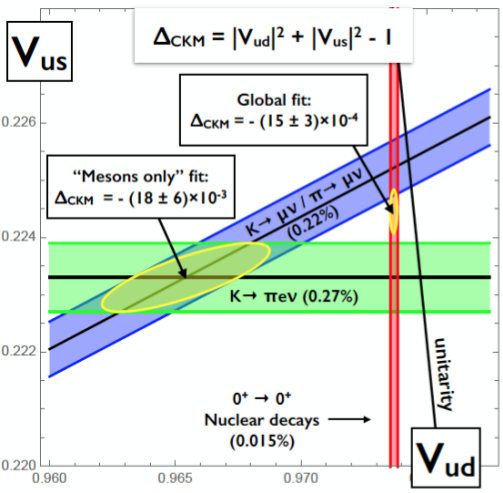
\includegraphics[scale=0.8]{sections/figures/fig-ckm.png}
\caption{Existing tensions in the 1st-row CKM unitarity test.}
\label{fig:CKM}
\end{figure}

